%%%%%%%%%%%%%%%%%%%%%%%%%%%%%%%%%%%%%%%%%
% Wenneker Assignment
% LaTeX Template
% Version 2.0 (12/1/2019)
%
% This template originates from:
% http://www.LaTeXTemplates.com
%
% Authors:
% Vel (vel@LaTeXTemplates.com)
% Frits Wenneker
%
% License:
% CC BY-NC-SA 3.0 (http://creativecommons.org/licenses/by-nc-sa/3.0/)
%
%%%%%%%%%%%%%%%%%%%%%%%%%%%%%%%%%%%%%%%%%

%----------------------------------------------------------------------------------------
%	PACKAGES AND OTHER DOCUMENT CONFIGURATIONS
%----------------------------------------------------------------------------------------

\documentclass[11pt]{scrartcl} % Font size
\usepackage{comment}
\usepackage{color}
%%%%%%%%%%%%%%%%%%%%%%%%%%%%%%%%%%%%%%%%%
% Wenneker Assignment
% Structure Specification File
% Version 2.0 (12/1/2019)
%
% This template originates from:
% http://www.LaTeXTemplates.com
%
% Authors:
% Vel (vel@LaTeXTemplates.com)
% Frits Wenneker
%
% License:
% CC BY-NC-SA 3.0 (http://creativecommons.org/licenses/by-nc-sa/3.0/)
% 
%%%%%%%%%%%%%%%%%%%%%%%%%%%%%%%%%%%%%%%%%

%----------------------------------------------------------------------------------------
%	PACKAGES AND OTHER DOCUMENT CONFIGURATIONS
%----------------------------------------------------------------------------------------

\usepackage{amsmath, amsfonts, amsthm} % Math packages
\usepackage{tabto}
\usepackage{listings} % Code listings, with syntax highlighting
\usepackage{tabu}
\usepackage{array}
\usepackage[english]{babel} % English language hyphenation
\usepackage{hyperref}

\usepackage{graphicx} % Required for inserting images
\graphicspath{{Figures/}{./}} % Specifies where to look for included images (trailing slash required)

\usepackage{booktabs} % Required for better horizontal rules in tables

\numberwithin{equation}{section} % Number equations within sections (i.e. 1.1, 1.2, 2.1, 2.2 instead of 1, 2, 3, 4)
\numberwithin{figure}{section} % Number figures within sections (i.e. 1.1, 1.2, 2.1, 2.2 instead of 1, 2, 3, 4)
\numberwithin{table}{section} % Number tables within sections (i.e. 1.1, 1.2, 2.1, 2.2 instead of 1, 2, 3, 4)

\setlength\parindent{0pt} % Removes all indentation from paragraphs

\usepackage{enumitem} % Required for list customisation
\setlist{noitemsep} % No spacing between list items

%----------------------------------------------------------------------------------------
%	DOCUMENT MARGINS
%----------------------------------------------------------------------------------------

\usepackage{geometry} % Required for adjusting page dimensions and margins

\geometry{
	paper=a4paper, % Paper size, change to letterpaper for US letter size
	top=2.5cm, % Top margin
	bottom=3cm, % Bottom margin
	left=3cm, % Left margin
	right=3cm, % Right margin
	headheight=0.75cm, % Header height
	footskip=1.5cm, % Space from the bottom margin to the baseline of the footer
	headsep=0.75cm, % Space from the top margin to the baseline of the header
	%showframe, % Uncomment to show how the type block is set on the page
}

%----------------------------------------------------------------------------------------
%	FONTS
%----------------------------------------------------------------------------------------

\usepackage[utf8]{inputenc} % Required for inputting international characters
\usepackage[T1]{fontenc} % Use 8-bit encoding

\usepackage{fourier} % Use the Adobe Utopia font for the document

%----------------------------------------------------------------------------------------
%	SECTION TITLES
%----------------------------------------------------------------------------------------

\usepackage{sectsty} % Allows customising section commands

\sectionfont{\vspace{6pt}\centering\normalfont\scshape} % \section{} styling
\subsectionfont{\normalfont\bfseries} % \subsection{} styling
\subsubsectionfont{\normalfont\itshape} % \subsubsection{} styling
\paragraphfont{\normalfont\scshape} % \paragraph{} styling

%----------------------------------------------------------------------------------------
%	HEADERS AND FOOTERS
%----------------------------------------------------------------------------------------

\usepackage{scrlayer-scrpage} % Required for customising headers and footers

\ohead*{} % Right header
\ihead*{} % Left header
\chead*{} % Centre header

\ofoot*{} % Right footer
\ifoot*{} % Left footer
\cfoot*{\pagemark} % Centre footer
 % Include the file specifying the document structure and custom commands
\usepackage{graphicx}
\usepackage{subcaption}



%Code retrieved from: https://www.overleaf.com/project/5c52d66b6343590b46b4fd03


%----------------------------------------------------------------------------------------
%	TITLE SECTION
%----------------------------------------------------------------------------------------

\title{
	\normalfont\normalsize
	\textsc{Old Dominion University}\\ % Your university, school and/or department name(s)
	\vspace{25pt} % Whitespace
	\rule{\linewidth}{0.5pt}\\ % Thin top horizontal rule
	\vspace{20pt} % Whitespace
	{\huge Assignment 8}\\ % The assignment title
	\vspace{12pt} % Whitespace
	\rule{\linewidth}{2pt}\\ % Thick bottom horizontal rule
	\vspace{12pt} % Whitespace
}

\author{\LARGE David Bayard} % Your name

\date{\normalsize\today} % Today's date (\today) or a custom date

\begin{document}

\definecolor{codegreen}{rgb}{0,0.6,0}
\definecolor{codegray}{rgb}{0.5,0.5,0.5}
\definecolor{codepurple}{rgb}{0.58,0,0.82}
\definecolor{backcolour}{rgb}{0.95,0.95,0.92}
\lstdefinestyle{pythonStyle}{
  backgroundcolor=\color{backcolour},
  commentstyle=\color{codegreen},
  keywordstyle=\color{magenta},
  numberstyle=\tiny\color{codegray},
  stringstyle=\color{codepurple},
  basicstyle=\footnotesize,
  breakatwhitespace=false,
  breaklines=true,
  captionpos=b,
  keepspaces=true,
  numbers=left,
  numbersep=5pt,
  showspaces=false,
  showstringspaces=false,
  showtabs=false,
  tabsize=2
}

\lstset{style=pythonStyle}


\maketitle % Print the title

\pagebreak
\section*{Question 1.}



%------------------------------------------------

\subsection*{Create two datasets; the first called Testing, the second called Training.}
\bigskip\bigskip


\large Solution:
\newline \small

\tabto{2.0cm} Two datasets were created by copying and pasting the text from 20 emails from the Spam folder, and another 20 from the inbox. Specific emails that contained certian query terms such as "ODU", or "Monarchs" were selected to increase
the odds of the classifier selecting the correct class per each document. Moreover, most of the emails shared a similar topic, being school related. This was purposefully done to test the classifier to a fuller extent.
\newline \newline

\tabto{2.0cm} The emails are split into two directories, being Spam and Not Spam. Within these directories, another two directories exist, called Test and Train. These folders represent the testing and training sets, containing 20 emails each. First, the training sets of Spam and Not Spam text files are run through the classifier, then the text files in the test directories are fed to the classifier. \newline

\section*{Question 2}


\subsection*{Using the PCI book modified docclass.py code and test.py (see Slack assignment-8 channel)
Use your Training dataset to train the Naive Bayes classifier ( e.g., docclass.spamTrain() )
Use your Testing dataset to test (test.py) the Naive Bayes classifier and report the classification results.}

%------------------------------------------------
\bigskip\bigskip
\LARGE Solution: \newline\newline\small

\tabto{2.0 cm} As specified above, the PCI book implements the Naive Bayes classifier functionality. Changes were made to the docclass.py file in order to read from the.txt files, instead of the SQLite database. Other then these changes, the original functions supplied by the PCI book were used as supplied. \newline \newline

\tabto{2.0cm} In order to train the Naive Bays classifier, three lines of code needed to be executed. First, an instance of the naivebays is instantiated and holds a reference to the getwords function. This is important becuase this function will later be used to extract all of the text from each of the .txt files, returning a lowercase count of each term. \newline \newline

\begin{lstlisting}[language = Python, caption=test.py driver function]
cl=docclass.naivebayes(docclass.getwords)

docclass.spamTrain(cl)
docclass.testClassifier(cl)
\end{lstlisting} \bigskip 

\tabto{2.0cm} When the naivebayes object is instantiated, a classifier object is created, and passed a reference the getwords function. In the function below, the spam files numbered from 1-11 are opened, and read into the InputStream, and then into strings. Every iteration, these strings are passed to the classifiers train method, which converts the words to lowercase, and keeps count of how many documents contain each word, and in which class they fall into. Sample output of this classification is shown below.

\begin{lstlisting}[language = Python, caption=Pass file input stream as string to classifier]

for r in range(1,11):
    spamFileName = "spamFile" + str(r)
    notSpamFileName = "notSpam" + str(r)
 
    spamFile = open("./Spam/Train/spam" + str(r) + ".txt", "r")
    notSpamFile = open("./Not_Spam/Train/NotSpam" + str(r) + ".txt", "r")
    text = spamFile.read()
    text2 = notSpamFile.read()

    cl.train(text2, "NotSpam")
    cl.train(text,'spam')

\end{lstlisting} \bigskip 


\begin{figure}[h!]
  \centering
  \begin{subfigure}[b]{\linewidth}
    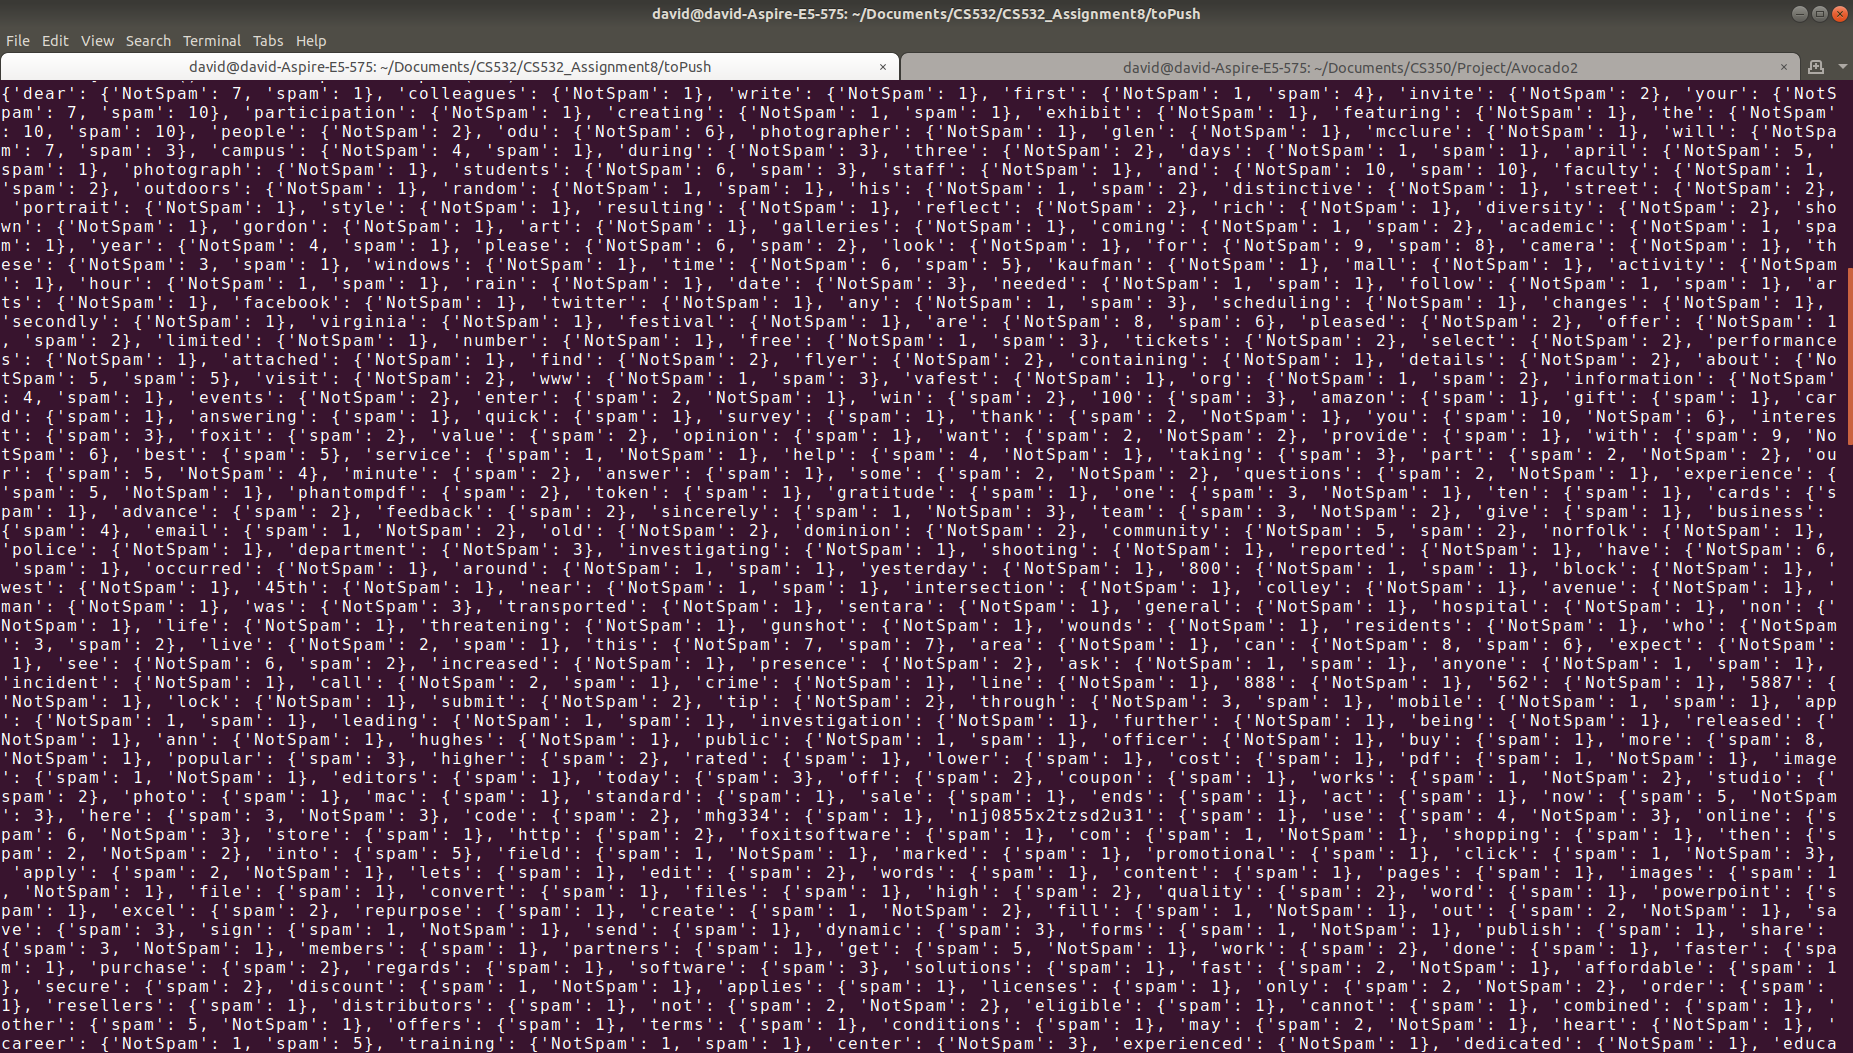
\includegraphics[width=\linewidth, height=.5\textheight]{../Figures/extractText.png}
    \caption{Extracting Text}
  \end{subfigure}
\end{figure}

\tabto{2.0cm} As seen in the image above, the words from all of the .txt files read in the function above are being extracted, transformed to lowercase, and counted. After the loop iterating over the files finishes running, the classifier object will contain each word in each document, a count of that word per document, and the class to which the word belongs. This data will be used when running the test files through the classifier to determine the correct class.
\pagebreak
  

\tabto{2.0cm} With the training data loaded into the classifier object, the testing data may now be loaded using the classify method in order to determine which class the test document belongs to. The code below loops over the remaining 20 documents, and predicts whether each documement is spam or not spam. 

\begin{lstlisting}[language = Python, caption= Clustering into 5 groups]
for r in range(11,21):

    spamFileName = "spamFile" + str(r)
    notSpamFileName = "notSpam" + str(r)
  
    spamFile = open("./Spam/Test/spam" + str(r) + ".txt", "r")
    notSpamFile = open("./Not_Spam/Test/NotSpam" + str(r) + ".txt", "r")
    text = spamFile.read()
    text2 = notSpamFile.read()

    predictNotSpam = cl.classify(text2, default='unknown')
    predictSpam = cl.classify(text,default='unknown')
\end{lstlisting}

\tabto{2.0cm} The results of the classify function, as well as a title line from each document are recorded in the documentation.txt file. From reading the documentation.txt file, it is visible that the classifier issued one false positive, classifying notSpam15.txt as spam. \newline \newline Overall, the classifier performed well, labeling 19 out of 20 documents in the proper class, but ranking the notSpam document as spam is a big mistake. This would be fixed by increasing the threshhold for a document to be classified as spam. While this may increase the odds of labeling spam documents as not spam, it helps prevent documents that are not spam from being labeled as spam.

\pagebreak


\section*{Question 3}

\subsection*{Draw a confusion matrix for your classification results}

%------------------------------------------------
\bigskip\bigskip
\LARGE Solution: \newline\newline\small


\tabto{2.0cm} The sklearn library is used here to draw the confusion matrix. It takes the true class values along with the predicted class values and draws the confusion matrix. \newline \newline In the confusion matrix shown below, the top left corner represents the properly selected spam class, and the bottom left row represents false positives of spam. Thus out of the 10 spam documents, 10 were properly predicted as spam, but 1 document was classified as spam when it is not spam.  \newline \newline The bottom right corner represents the documents that are not spam. The classifier predicted only 9 documents as not spam, and the top right row displaying false negatives remains empty.

\begin{figure}[h!]
  \centering
  \begin{subfigure}[b]{\linewidth}
    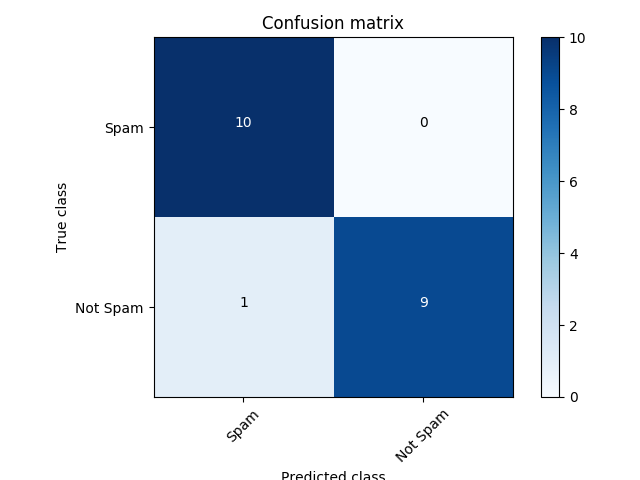
\includegraphics[width=\linewidth, height=.5\textheight]{../Figures/confusionMatrix.png}
  \end{subfigure}
\end{figure}



\pagebreak

\section*{Question 4}


\subsection*{Report the precision and accuracy scores of your classification results}

%------------------------------------------------
\bigskip\bigskip
\LARGE Solution: \newline\newline\small

\tabto{2.0 cm} The formulas necessary to calculate the accuracy and precision are displayed below.

$$ Precision = \frac{tp}{tp + fp}$$
$$ Accuracy = \frac{tp + tn}{tp + tn + fp + fn} $$

\bigskip \bigskip

\tabto{2.0cm} The equations above represent tp as true positive, fp = false positive, tn as true negative, and  fn as false negative. The equations are filled in with the values from the confusion matrix.

\bigskip
$$ Precision = \frac{10}{10+1} = \frac{10}{11} = .91$$
$$ Accuracy = \frac{10 + 9}{9+10+1+0} = \frac{19}{20} = .95 $$
\bigskip \bigskip

\tabto{2.0cm} As seen above, the classifier has a fairly high precision and accuracy. These values would undoubtedly change given a larger sample size, but for a sample of only 20 files, the values are reasonable.




\end{document}
